
\chapter{Referencial Teórico}

% Começando do básico do básico do básico

Computadores são sistemas incrivelmente complexos. Inúmeros componentes com
papeis específicos necessitam de se intercomunicar para executar a mais simples
das tarefas. Dessa forma, para compreender seu funcionamento, se faz o uso de
camadas de abstrações.

% Camadas de abstrações
Essas camadas exercem funções diferentes e são visíveis de acordo com seu uso
--- um usuário final não precisa saber programar para usar um processador de
texto; da mesma forma, um programador não necessita saber da estrutura dos
circuitos internos. Cada camada possui seu domínio, sendo as mais próximas do
usuário final denominadas de ``alto-nível'' e as mais próximas dos transistores
e fios, ``baixo-nível''. Observe a figura \ref{camadas}, especificada de acordo
com Murdocca \cite{principles}.

% As várias camadas bonitinhas
\begin{figure}[ptb]
  \begin{center}
    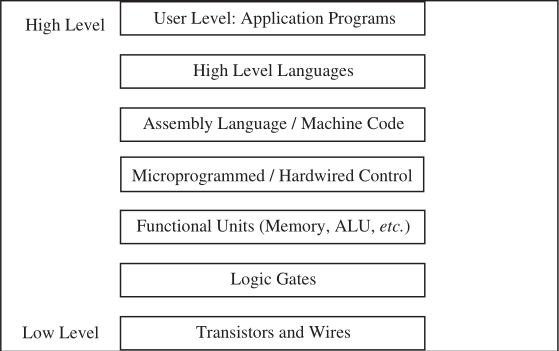
\includegraphics[scale=.6]{imagens/1_camadas}
  \end{center}
  \caption{Camadas de abstração de um computador.}
  \label{camadas}
\end{figure}

Iremos definir conceitos básicos, utilizados ao longo do trabalho. Nossa
abordagem será \textit{top-down}, significando que os conceitos serão explicados
do nível mais abstrato até o mais concreto nível de \textit{hardware}.

\section{Arquitetura de Processadores}

\section{Redes de Computadores}

CPU

\section{Teoria da Codificação e Criptografia}

CPU

\section{Tradutores}

% Importância de Compiladores
No âmbito da computação em geral, compiladores são uma das mais importantes
aplicações.  É impossível imaginar um sistema computacional sem alguma forma de
compilação. Compiladores estão presentes em quase todas as camadas de abstração
de um computador.

% Calma aê, vamos começar lá de cima
Porém, para compreender o conceito de compilador é necessário estudar sobre
linguagens de programação e o processo de tradução.

\subsection{Linguagens}

% Linguagem é muito abstrato
% CITAR COISA ABSTRATA SOBRE LINGUAGENS
\textit{Linguagem} é um conceito abrangente. Enquanto que diferentes áreas do
conhecimento definam \textit{linguagem} por formas específicas, para nosso
trabalho será suficiente uma definição geral.

% OK, lá vai... Linguagem
Linguagem é um sistema de comunicação - um conjunto de regras e convenções que
permitem a interação entre dois pares. Dialetos humanos (português, inglês,
francês...) são exemplos de tais sistemas de comunicação. Cada um destes define
acordos (gramáticas, sintaxe, morfologia) que permitem a troca de mensagens
entre pessoas de mesmo grupo.

% Coisas interessantes sobre linguagem
Dessa forma, pares que queiram interagir entre si necessitarão de trocar
conhecimento através de mensagens na mesma linguagem. Caso haja comunicação por
duas linguagens diferentes, ocorrerão erros de compreensão, desentendimentos e
até completa inabilidade de se comunicar.

\subsection{Linguagens de Programação}

% Linguagem de programação
Partindo para o domínio computacional, há o conceito de linguagens de
programação. Estas possuem objetivo de comunicar instruções de seres humanos
para máquinas. Mais especificamente, possuem o objetivo de determinar o que
computadores devem fazer - como estes são programados a agir.

% Programação -> Máquina
Linguagens de programação são destinadas a expressar idéias concebidas por seres
humanos. Dessa forma, precisam se aproximar da linguagem natural - forma de
comunicação natural entre seres humanos.  Devido à construção física de
máquinas, computadores precisam de instruções em formato bastante diferente do
oferecido pela linguagem natural - quanto mais de linguagens de programação.

\subsection{Linguagem de Máquina}

% Linguagem de máquina
É nesse conceito que se define a linguagem de máquina, também conhecida como
código de máquina. São conjuntos de instruções (ou ordens) que determinam como a
máquina irá se comportar. Controla-se um computador ao agrupar várias dessas
instruções em ordens específicas.

% Não é linguagem de programação
Linguagem de máquina se diferencia das linguagens de programação no sentido de
que não são facilmente compreendidas por seres humanos. Enquanto que linguagens
de programação se aproximam da linguagem natural, linguagem de máquina é
definida pela construção física dos componentes de cada máquina.

Observaremos mais detalhes sobre linguagem de maquina na seçao
\ref{subsec:linguagem_maquina}.

\subsection{Linguagens de Alto e Baixo nível}

% Linguagens de alto-nível e baixo-nível, exemplos
Com linguagens em pontos tão extremos, como alto e baixo nível, se torna
impossível a comunicação entre pares que as utilizem. Necessita-se de um meio de
conversão entre estas.

\subsection{Tradução}

% Tradução - duas linguagens % CITAR COISA ABSTRATA SOBRE LINGUAGENS

% Exemplos de tradução

\subsection{Compiladores}

% Finalmente, compiladores
% CITAR CONCEITO DE COMPILADORES
Compiladores são programas que transformam código-fonte escrito em uma linguagem
de programação em outra. Eles fazem o processo de tradução, em geral de
linguagens de alto nível para linguagens de baixo-nível.

\section{Software Básico}

Na seção anterior, descrevemos os conceitos básicos necessários para compreender
como se dá a criação de um programa de computador, que pode ser por exemplo um
\textit{software} de aplicação. Geralmente classificamos os programas utilizados
por usuários finais como \textit{software} de aplicação.

Programas tradutores como os descritos na seção anterior são classificados como
\textit{software} básico, ou \textit{software} de sistema. Dizemos que
\textit{software} básico faz parte de um conjunto de \textit{softwares}, ou de
um sistema, capaz de gerenciar a utilização do \textit{hardware} de modo a
fornecer uma plataforma para \textit{softwares} de aplicação (uma ref. aqui).

Entre os tipos de \textit{software} classificados como \textit{software} básico,
podemos incluir tradutores (como compiladores e montadores), ligadores, sistemas
operacionais (que incluem carregadores e \textit{drivers} de dispositivos) e
sistemas embarcados (uma ref. aqui). Discutiremos sistemas operacionais na
próxima seção.

\subsection{Linguagem de Máquina}
\label{subsec:linguagem_maquina}

Anteriormente vimos que uma linguagem de montagem, ou linguagem
\textit{assembly}, é formada por símbolos mnemônicos, ou palavras-chave, que
identificam as instruções que um processador é capaz de executar.

A etapa seguinte à compilação é a montagem. Nesta etapa, é necessário traduzir
os mnemônicos \textit{assembly} para sequências de \textit{bits}. Um
\textit{bit} é um dígito que pode assumir apenas o valor 0 (zero) ou o valor 1
(um). Durante a execução de um programa, estas sequências de \textit{bits} serão
diretamente interpretadas por uma \textit{CPU}.

Costuma-se dizer que a etapa de montagem é onde está localizada a interface
\textit{software}-\textit{hardware}. Uma \textit{ISA} - \textit{Instruction Set
Architecture}, ou Arquitetura de Conjunto de Instruções - é uma especificação
das instruções que uma implementação de processador digital deve fornecer. Esta
especificação, entre outras coisas, estabelece os formatos que as sequências de
\textit{bits} geradas por montadores devem seguir. Este é o principal
conhecimento necessário para construir um montador.

A figura \ref{instrucoes_mips} mostra os três formatos principais de instruções
da arquitetura \textit{RISC} \textit{MIPS32} (uma ref. aqui). Grandes
quantidades de instruções se encaixam em cada um dos três formatos. Nesta
arquitetura, toda e qualquer instrução ocupa uma palavra de 32 \textit{bits}.

\begin{figure}[ptb]
  \begin{center}
    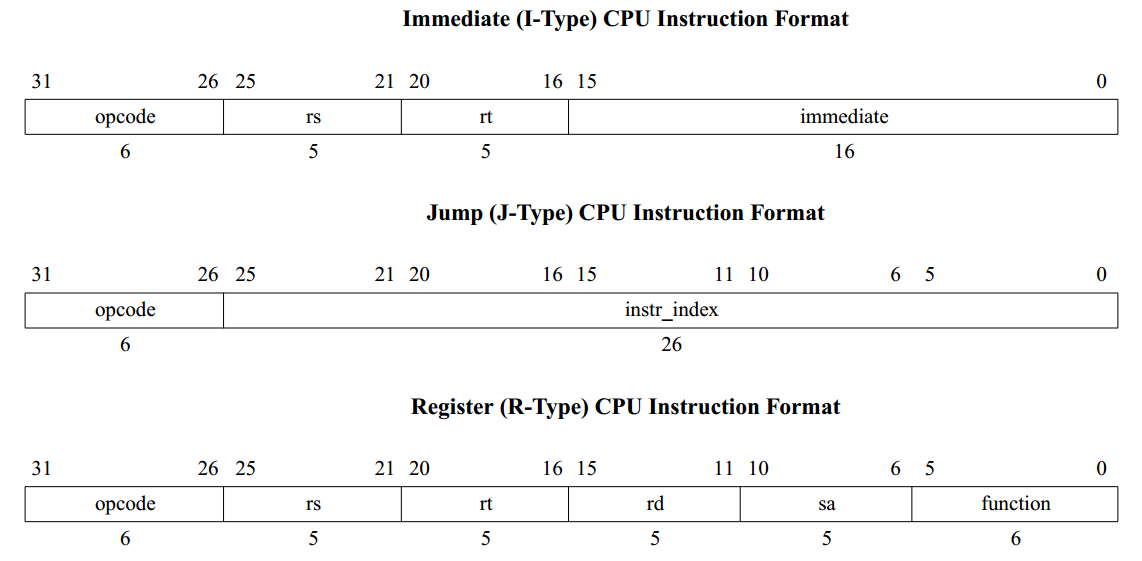
\includegraphics[scale=.35]{imagens/instrucoes_mips}
  \end{center}
  \caption{Os três formatos principais da \textit{ISA} \textit{MIPS32}.}
  \label{instrucoes_mips}
\end{figure}

A figura \ref{instrucoes_ia32} mostra o formato geral para uma instrução
qualquer da arquitetura \textit{CISC} \textit{IA-32} (uma ref. aqui), criada
pela Intel. Nesta arquitetura, o tamanho das instruções vai de 1 até 17
\textit{bytes} (um \textit{byte} são exatamente 8 \textit{bits}).

\begin{figure}[ptb]
  \begin{center}
    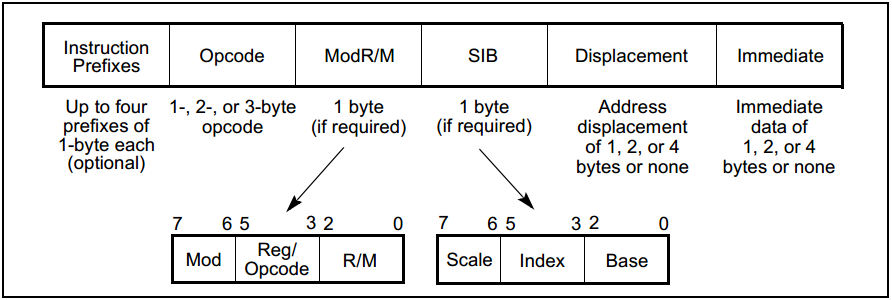
\includegraphics[scale=.45]{imagens/instrucoes_ia32}
  \end{center}
  \caption{Formato geral de uma instrução da \textit{ISA} \textit{IA-32}.}
  \label{instrucoes_ia32}
\end{figure}

Com o conhecimento de como cada mnemônico deve ser convertido para código de
máquina, podemos construir um montador para uma determinada arquitetura de
processadores. À seguir descrevemos os algoritmos clássicos de montagem.

\subsection{Montadores}

Montadores são programas que traduzem um módulo de compilação em linguagem
\textit{assembly} para uma versão em linguagem de máquina. O armazenamento desta
versão é feito em um arquivo objeto. Como veremos em uma subseção adiante, um
arquivo objeto é uma versão binária de um módulo de compilação, que geralmente
fica a um passo de poder ser carregada para execução.

O problema da montagem pode ser colocado da seguinte forma: um módulo de
compilação em linguagem \textit{assembly} contém dados e instruções mnemônicas
que devem ser convertidas para binário seguindo a ordem em que aparecem. Para
termos a noção de localização de um dado ou instrução, temos o conceito de
endereço de memória.

Antes de definirmos o conceito de endereço de memória, precisamos definir o
conceito de palavra. Uma palavra é um agrupamento de uma quantidade fixa de
\textit{bits}. Uma \textit{ISA} determina os diferentes tamanhos de palavras que
podem ser utilizados para escrever um programa. Geralmente, o menor tamanho de
palavra suportado é o \textit{byte}, enquanto os outros tamanhos costumam ser
múltiplos em potência de 2 de um \textit{byte}.

Aqui iremos nos referir a um endereço de memória como um número cuja unidade é o
menor tamanho de palavra definido por uma arquitetura. Para referenciar
endereços, linguagens de montagem costumam utilizar o que chamamos de símbolo,
ou rótulo. Um símbolo pode ser uma palavra ou uma frase de linguagem natural.

Para realizar a conversão de um arquivo \textit{assembly} para binário, é
necessário que um algoritmo de montagem realize passagens no arquivo de entrada,
coletando informações de montagem. Com informação suficiente, o montador é capaz
de colocar os dados em determinados endereços, colocar as instruções na ordem em
que aparecem em outros endereços e substituir ocorrências de rótulos por seus
respectivos endereços.

A próxima subseção descreve o algoritmo de duas passagens, o mais trivial.

\subsection{Montadores de duas passagens}

Na primeira passagem pelo código \textit{assembly}, um algoritmo de duas
passagem cria uma tabela de símbolos.

A tabela de símbolos é uma estrutura indexada por símbolos (ou rótulos). Para
cada símbolo que indexar a tabela, temos uma entrada com o endereço ao qual o
símbolo se refere e algumas informações adicionais. É criada uma entrada nesta
tabela para cada rótulo que for encontrado no código-fonte. Rótulos podem ser
criados tanto para dados, quanto para instruções.

Em um programa \textit{assembly}, símbolos podem estar presentes tanto em
definições de símbilos, ou seja, em locais onde o endereço de um símbolo é
estabelecido, quanto podem estar contidos em instruções que referenciam
endereços através de símbolos. Ao encontrar a definição de um símbolo, o
montador pode gerar um erro, ou aviso, caso este símbolo já tenha sido definido
anteriormente. Se a definição de um símbolo declara um dado, o montador pode
colocar esta informação na entrada da tabela de símbolos.

Um montador tem a liberdade de implementar funcionalidades que facilitam a vida
de um programador \textit{assembly}. Uma funcionalidade comumente implementada é
a disponibilização de diretivas de pré-processamento. Diretivas são instruções
ao próprio montador, ou seja, diretivas não são instruções que geram código de
máquina.

Outra funcionalidade comum, é a utilização de
pseudo-instruções. Pseudo-instruções utilizam mnemônicos e formatos parecidos
com os das instruções concretas da \textit{ISA}, mas são instruções que não
estão de fato implementadas em \textit{hardware}. É comum montadores fornecerem
pseudo-instruções que expandem para muitas instruções concretas, que em conjunto
realizam uma tarefa mais complexa.

Ainda na primeira passagem, o montador pode avaliar mnemônicos de instruções. Ao
avaliar uma instrução, o montador pode gerar um erro caso não identifique o
mnemônico da operação como válido. Um mnemônico válido pode ser o de uma
instrução concreta, o de uma pseudo-instrução, ou pode ser uma diretiva de
pré-processamento.

Com a tabela de símbolos pronta, o montador pode realizar a segunda
passagem. Esta é a etapa em que o montador de fato gera código de máquina.

O montador examina cada instrução à procura de símbolos. Símbolos que não
estejam presentes na tabela de símbolos geram erro de montagem. Para instruções
com símbolos definidos, o montador gera o código de máquina correspondente,
substituindo cada símbolo por seu respectivo endereço.

Ao final da segunda passagem, o montador está pronto para gerar o arquivo
objeto. Nesta etapa, coloca-se o código de máquina gerado junto com um espaço
alocado para dados. Ao gerar de fato o arquivo de saída, o montador coloca nele
informação de relocação, uma tabela de símbolos exportados e uma tabela de
referências externas.

A figura \ref{duas_passagens} ilustra a execução de um algoritmo de duas
passagens sobre um código \textit{assembly} hipotético (uma ref. aqui).

Voltaremos agora nossa atenção ao algoritmo de passagem única, desenvolvido para
ser mais eficiente do que o algoritmo que acabamos de descrever. Iremos deixar a
discussão sobre arquivos objeto para a subseção depois da próxima.

\begin{figure}[ptb]
  \begin{center}
    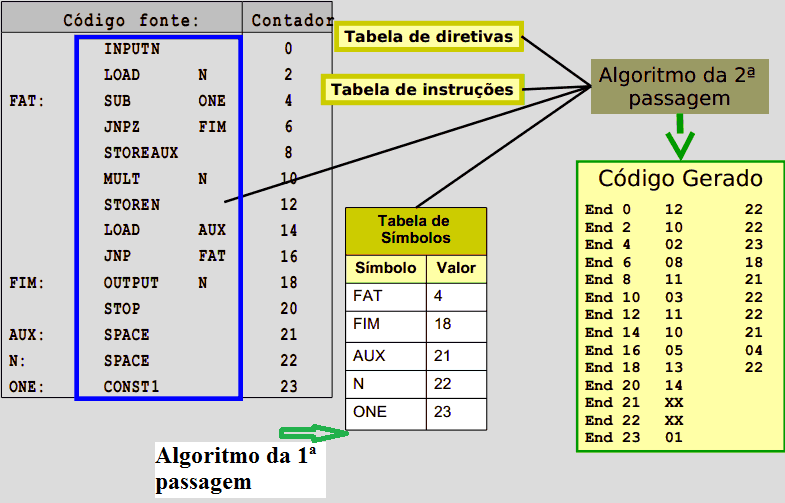
\includegraphics[scale=.7]{imagens/duas_passagens}
  \end{center}
  \caption{Ilustração do algoritmo de duas passagens sobre um \textit{assembly}
hipotético.}
  \label{duas_passagens}
\end{figure}

\subsection{Montadores de passagem única}

O algoritmo de passagem única pode ser considerado uma evolução do algoritmo
descrito acima.

Um montador de passagem única constrói a tabela de símbolos ao passo que gera
código de máquina. Para trabalhar desta forma, são necessárias listas de
referências pendentes.

Para cada símbolo encontrado em uma instrução que não estiver presente na tabela
de símbolos, o algoritmo cria uma entrada na tabela, marca o símbolo como
indefinido e cria uma lista de referências àquele símbolo.

Ao encontrar a definição de um símbolo, montadores de passagem única ainda geram
erro, caso o símbolo já tenha sido definido anteriormente. No entanto, se o
símbolo é encontrado na tabela, mas está marcado como indefinido, o algoritmo
marca este símbolo como definido, estabelece seu endereço e itera sobre a lista
de referências àquele símbolo atualizando os campos com o endereço válido. A
implementação de um montador pode escolher atualizar as referências ao final da
passagem, ao invés de realizar esta tarefa imediatamente.

Após a passagem ser realizada, se ainda existirem símbolos indefinidos o
montador gera erro. O restante do processo é o mesmo que o descrito no algoritmo
de duas passagens.

\subsection{Arquivos objeto}

Chamamos a saída de um montador de arquivo objeto. Juntamente com o código de
máquina montado, montadores geram informações necessárias para etapas seguintes,
até que o programa possa de fato ser executado em uma \textit{CPU}.

Uma das estruturas colocadas em um arquivo objeto é uma lista de
relocação. Anteriormente definimos o que são endereços. Agora vamos definir o
que são endereços absolutos e o que são endereços relativos.

Uma lista de relocação armazena endereços absolutos. Endereços absolutos são
endereços calculados utilizando um endereço base. Relocação é o processo de
somar um endereço base à um endereço absoluto. Pode-se considerar que, durante a
montagem, o endereço base é o endereço zero. Na subseção que vem à seguir,
veremos mais sobre relocação.

Em contrapartida, endereços relativos são endereços que não precisam de
relocação, pois são endereços cujo endereço base é a própria posição da
instrução. Veremos mais sobre endereços relativos na próxima subseção.

Outra estrutura gerada por um montador é uma tabela de símbolos exportados. Ao
definir um símbolo em um módulo de compilação, podemos querer referenciá-lo de
outro módulo de compilação. Para que isto seja possível, é necessário declarar
quais símbolos de um módulo serão exportados. A subseção à seguir trata sobre
este assunto.

A terceira e última estrutura presente na saída de um montador é uma tabela de
referências externas. Esta é a recíproca da tabela de símbolos exportados. Ao
mesmo tempo que um módulo de compilação pode fornecer símbolos a serem
referenciados em outros módulos, este mesmo módulo obviamente deve conter
informações que dizem aonde símbolos externos foram utilizados. A tabela de
referências externas contém listas de referências para cada símbolo importado.

Após criar uma seção inicial no arquivo binário que contém estas informações,
seção que geralmente é denominada como cabeçalho, o montador coloca na saída o
código de máquina montado. A etapa seguinte à montagem é ligação.

\subsection{Ligadores}

Após arquivos objeto de um ou vários módulos de compilação serem gerados por um
montador, é preciso combiná-los em um único arquivo que pode ser carregado para
a memória por um programa carregador do sistema operacional.

Ligadores utilizam as três informações colocadas nos cabeçalhos de arquivos
objeto para gerar arquivos executáveis, ou bibliotecas de código.

Arquivos executáveis, ou módulos de carga, são arquivos que estão quase prontos
para serem carregados na memória de um computador e serem executados. A etapa
final que pode estar faltando é a relocação de endereços absolutos, caso o
programa utilize instruções com este tipo de endereçamento. Discutiremos o
processo de carga na próxima subseção.

Bibliotecas de código são arquivos com código de máquina que reúnem diversas
funcionalidades e podem ser aproveitadas por outros programas. Bibliotecas
dividem-se em bibliotecas estáticas e bibliotecas dinâmicas.

Bibliotecas estáticas são a combinação de vários arquivos objeto que utilizam
instruções de máquina com endereços absolutos. Desta forma, para um programa
aproveitar uma biblioteca estática, basta que o ligador considere esta
biblioteca como um simples arquivo objeto. Portanto, é claro que o ligador
também é responsável por gerar informações de relocação, símbolos e referências
externas.

Bibliotecas dinâmicas, também consideradas módulos de carga, são a combinação de
vários arquivos objeto que utilizam instruções de máquina com endereços
relativos. A vantagem de se utilizar endereços relativos é que o módulo de carga
pode ser carregado em qualquer posição da memória, sem que relocação seja
necessária. Outra vantagem de utilizar bibliotecas dinâmicas, é a produção de
arquivos executáveis mais leves. Em alguns sistemas operacionais, apenas uma
cópia de uma biblioteca dinâmica na memória é necessária para a execução
simultânea de diversos programas.

Neste ponto, deve estar fácil de concluir que ligadores aceitam como entrada não
apenas arquivos objeto, como aceitam também bibliotecas.

O processo de ligação é extremamente simples. A primeira tarefa a ser realizada
na ligação é o carregamento dos arquivos de entrada em uma determinada ordem. A
cada arquivo carregado, o algoritmo de ligação associa um endereço base de
posicionamento. Este endereço base é utilizado para relocar todas as instruções
de endereçamento absoluto daquele arquivo.

Após carregar, colocar juntos os arquivos de entrada e efetuar as relocações, o
algoritmo de ligação une as tabelas de símbolos exportados de cada arquivo em
uma grade tabela global de símbolos.

Com a tabela global de símbolos, é possível passar pelas referências externas de
cada arquivo, preenchendo cada campo com o respectivo endereço.

Na criação de uma biblioteca estática, o ligador deve gerar uma nova lista de
relocação, utilizar a tabela global de símbolos como a nova tabela de símbolos
exportados e pode criar uma nova tabela de referências pendentes, caso nem todas
as referências tenham sido resolvidas durante aquela ligação. Na criação de uma
biblioteca dinâmica, informação de relocação não é gerada.

Ao criar um arquivo executável, o ligador pode gerar informação de relocação e
uma tabela de referências externas (para o caso de ligação com bibliotecas
dinâmicas). Além disso, o ligador espera que um dos arquivos de entrada exporte
um símbolo especial que possa ser estabelecido com o ponto de entrada do
programa. Esta é uma regra imposta por formatos de arquivos executáveis,
adotados por sistemas operacionais.

Na prática, um ligador quase sempre gera uma tabela de referências externas em
arquivos executáveis, pois diversos sistemas operacionais estabelecem que a
própria biblioteca dinâmica que implementa operações de ligação deve ser ligada
com um programa, obviamente para que seja possível realizar ligações com
bibliotecas dinâmicas. A utilização de bibliotecas dinâmicas implica na
necessidade de realizar relocação em tempo de execução, pois um sistema
operacional pode determinar que uma biblioteca só deve ser carregada quando for
de fato chamada (uma ref. aqui).

Com os dados de cabeçalho prontos, o ligador finalmente gera um arquivo binário
com código de máquina. À seguir, descrevemos o processo de carregamento de
módulos de carga para execução.

\subsection{Carregadores}

CPU

\section{Sistemas Operacionais}

CPU

\section{Organização e Arquitetura de Computadores}

CPU

\subsection{Arquitetura de Processadores Digitais}

CPU

\subsection{Controladores de Dispositivos Externos}

CPU

\section{Circuitos Digitais}

CPU

\subsection{Lógica Booleana e Circuitos Combinacionais}

CPU

\subsection{Circuitos Sequenciais}

CPU

\subsection{Arranjo de Portas Programável em Campo}

CPU

\subsection{Linguagem de Descrição de Hardware}

CPU

